\chapter{Flow Control}
In this chapter, implementation and evaluation of various control algorithms for flow control purposes will be presented. At first, the aim is to enable regulation of flow to a constant value. Later on, the system's ability to follow different reference flow trajectories will be tested. In a final step, the system will be subjected to disturbances through the HiL test rig in form of heart beats at different heart rates. Performances of the implemented control algorithms will be compared.
% As a first step towards flow control implementation two versions of PI controllers are implemented to ensure stable system behavior. After comparing the performance results of both approaches, a parallel approach to ILC implementation under use of the higher performing PI controller is applied to improve the follow up behavior and reduce control errors.
\section{PI Controller}
PI control implementation is performed on the basis of the tuning rules according to Ziegler Nichols as well as according to Chien Hrones Reswick (Chapter \ref{chap:CHR}). The performance of both controllers later on is  compared and evaluated.
\subsection{Design and Implementation}
As a preparation for utilization of the inflection tangent method for these tuning approaches, a measurement similar to the one for determining the static map is performed. \figurename~\ref{fig:dyn_meas} depicts the signal curves for determination of the tuning parameters.
\begin{figure}[ht]
  \centering
  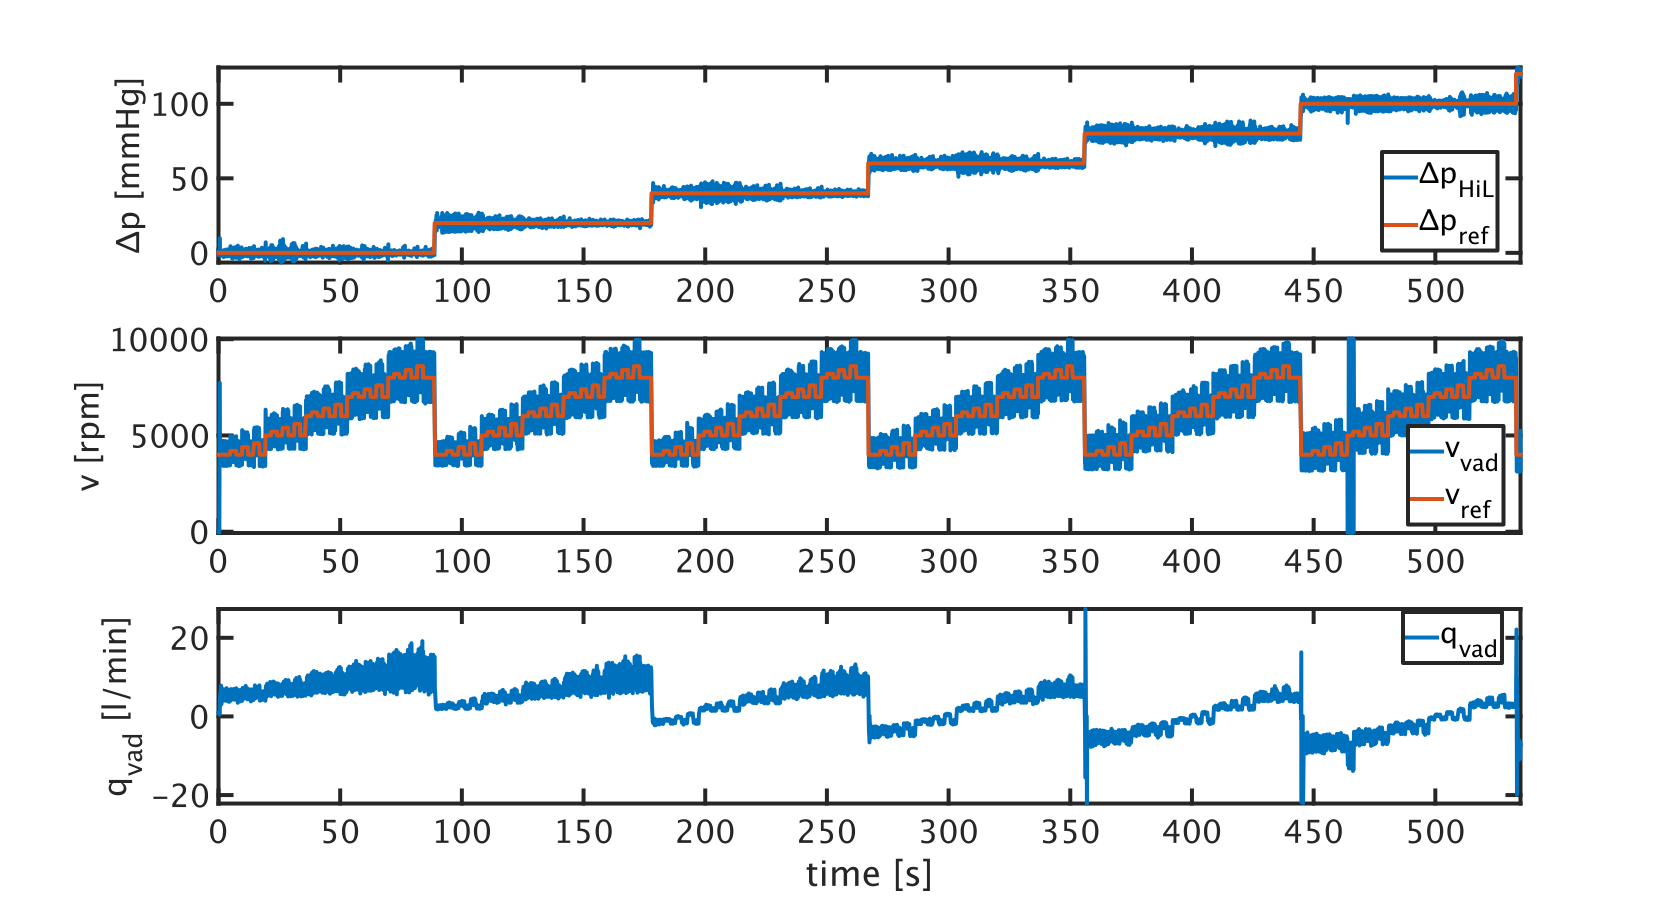
\includegraphics[width=\textwidth]{images/chapt_5/dyn_measure.pdf}
  \caption[Signal curves for determination of PI controller parameters]{Signal curves for determination of PI controller parameters. Top: differential pressure as reference and measured signal, middle: reference and measured rotational speed, bottom: measured flow through Sputnik VAD.}
  \label{fig:dyn_meas}
\end{figure}
As presented in the upper graph, differential pressure is increased in steps of $20\,mmHg$ from $\Delta{p}=0\,mmHg$ to $\Delta{p}=100\,mmHg$. For each level the sequence of reference velocities depicted exemplary for $\Delta{p}=40\,mmHg$ in the center graph of \figurename~\ref{fig:dyn_meas_40} is targeted. Starting at $v_{ref}=4000 \, rpm $ the velocity is first increased in three steps of varying height and then decreased by the same values. The first step amounts to $200 \, rpm$, the second to $400\,rpm$ and the third to $600 \, rpm$. The reference value is then increased by $1000\,rpm$ and again the three steps are executed. This sequential behavior is repeated up to a start value of $v_{ref}=8000\,rpm$.
\begin{figure}[ht]
  \centering
  \includegraphics[width=\textwidth]{images/chapt_5/dyn_meas_40.pdf}
  \caption[Signal curves for determination of PI controller parameters at $\Delta{p}=40\,mmHg$]{Signal curves for determination of PI controller parameters at $\Delta{p}=40\,mmHg$.}
  \label{fig:dyn_meas_40}
\end{figure}
For determination of the parameters for controller design the step from $v_{ref,low}=5000\, rpm$ to $v_{ref,high}=5400\, rpm$ at $\Delta{p}=40\,mmHg$, which is located in the center of the pump's operating range, is used.
Since the flow signal is affected by high measurement noise, the signal is preprocessed using an $8^{th}$-order butterworth filter with cut off frequency $f_c=5\,Hz$ and sampling frequency $f_s=1000\,Hz$.
\begin{figure}[ht]
  \centering
  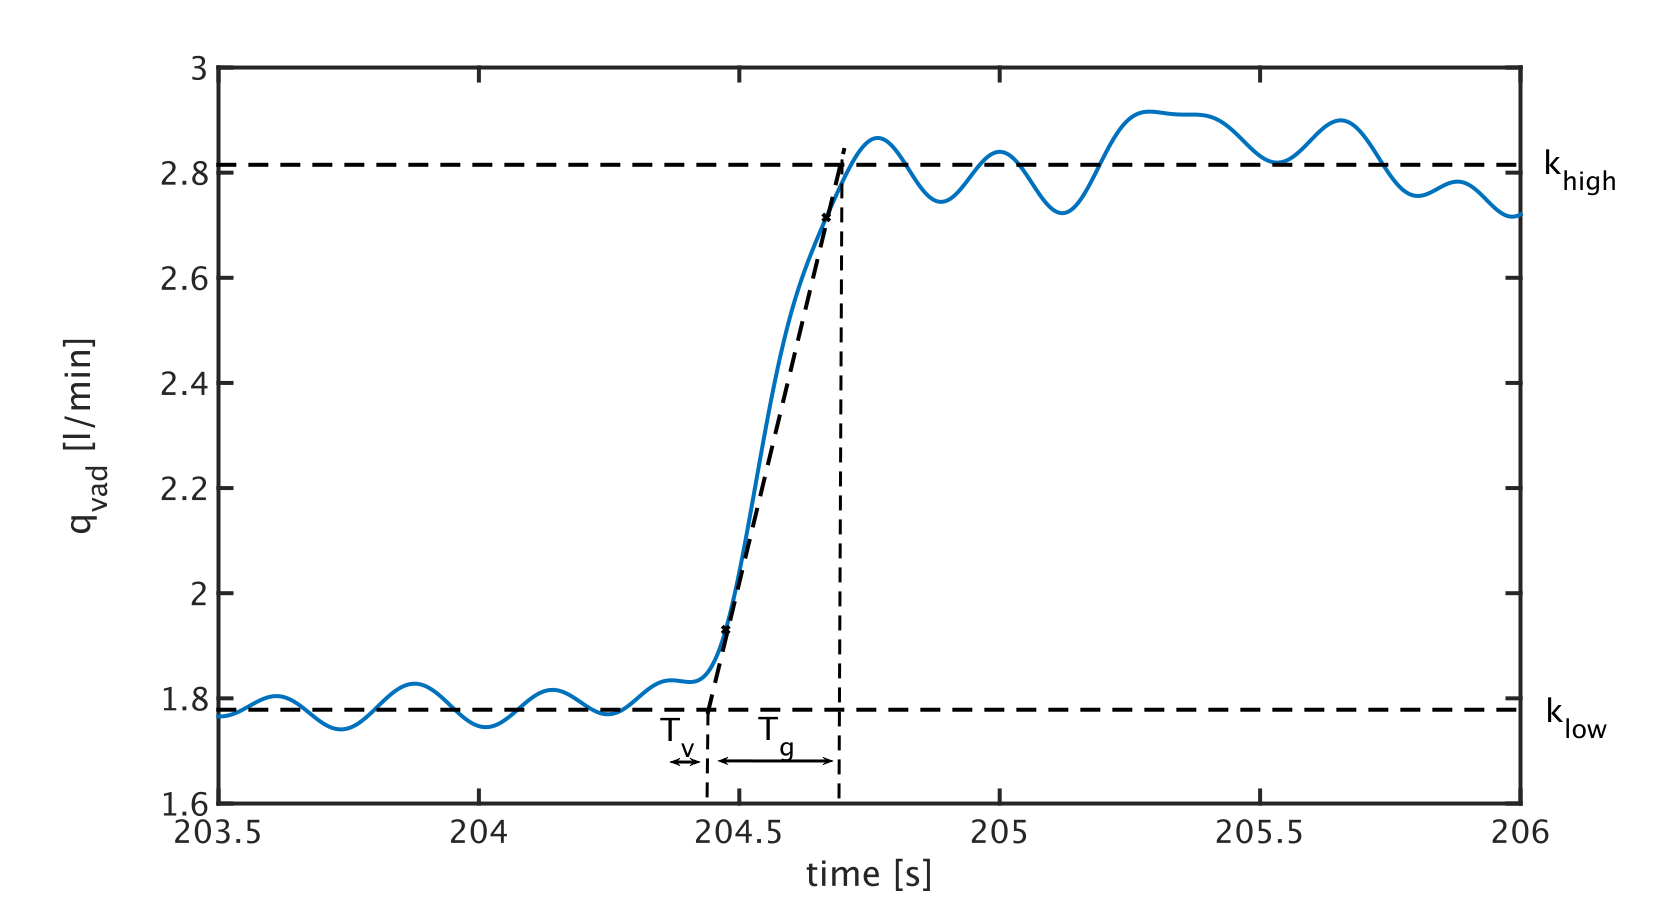
\includegraphics[width=\textwidth]{images/chapt_5/param_calc_PI.pdf}
  \caption[Step response for determination of PI controller tuning parameters]{Step response for a step in rotational speed of $400\,rpm$ for determination of PI controller tuning parameters.}
  \label{fig:param_calc_PI}
\end{figure}
The resulting signal and the characteristic parameters needed for parameter tuning of the PI controller are depicted in \figurename~\ref{fig:param_calc_PI}. With $k_{high}=2.8149$ and $k_{low}=1.7783$ the static gain is determined as in equation (\ref{eq:k_s_1}) to
\begin{equation}
  k_s = \frac{k_{high}-k_{low}}{v_{ref,high}-v_{ref,low}}= 0.0026.
\label{eq:k_s_2}
\end{equation}
The time constants amount to $T_g=0.193$ and $T_v=0.1$.
\\For determination of a PI controller tuned according to Ziegler Nichols equations (\ref{eq:kp_zn}) to (\ref{eq:T_N_zn}) are used. By this $K_{P}$ is determined as
\begin{equation}
  K_{P} = 0.9*\frac{0.193}{0.0026*0.1}=670.3052
\end{equation}
and $K_I$ as
\begin{equation}
  K_{I}  = \frac{670.3052}{3.3*0.1}=2031.2278.
\end{equation}
Substituting these values in equation (\ref{eq:pi_contr_2}) results in the transfer function
\begin{equation}
  G_{PI,ZN}(s)=670.3052+\frac{2031.2278}{s}.
\end{equation}
\\Calculation for overdamped controller behavior was chosen for controller tuning using Chien Hrones Reswick. Determination of the parameters $K_P$ and $K_I$ is performed following the equations presented in \tablename~\ref{tab:param_chr}, resulting in
\begin{equation}
  K_P = 0.35*\frac{0.193}{0.0026*0.1}=260.6742
\end{equation}
and
\begin{equation}
  K_I = \frac{260.6742}{1.2*0.1}=2172.2853.
\end{equation}
This in turn leads to the transfer function
\begin{equation}
  G_{PI,CHR}(s)=260.6742+\frac{2172.2853}{s}.
\end{equation}
\subsection{Evaluation}
The main purpose for utilization of a PI controller, in this work, is to stabilize the closed loop signal behavior in preparation for an ILC implementation.
Both controllers are therefore tested under the same operating conditions and their performance is compared.
\\Even though the controllers are tuned at $\Delta{p}=40\,mmHg$, both of them  are tested in the differential pressure operating range from $\Delta{p}=0\,mmHg$ to $\Delta{p}=100\,mmHg$ to ensure sufficient performance in all use cases.
For each differential pressure level three consecutive steps up and down throughout the operating range of flow are performed. Each reference flow is targeted for $5\,s$ and flow through the VAD is measured. A graphical representation of the reference signal curves is depicted in \figurename~\ref{fig:PI_control_ref_signals}.
\begin{figure}[ht]
  \centering
  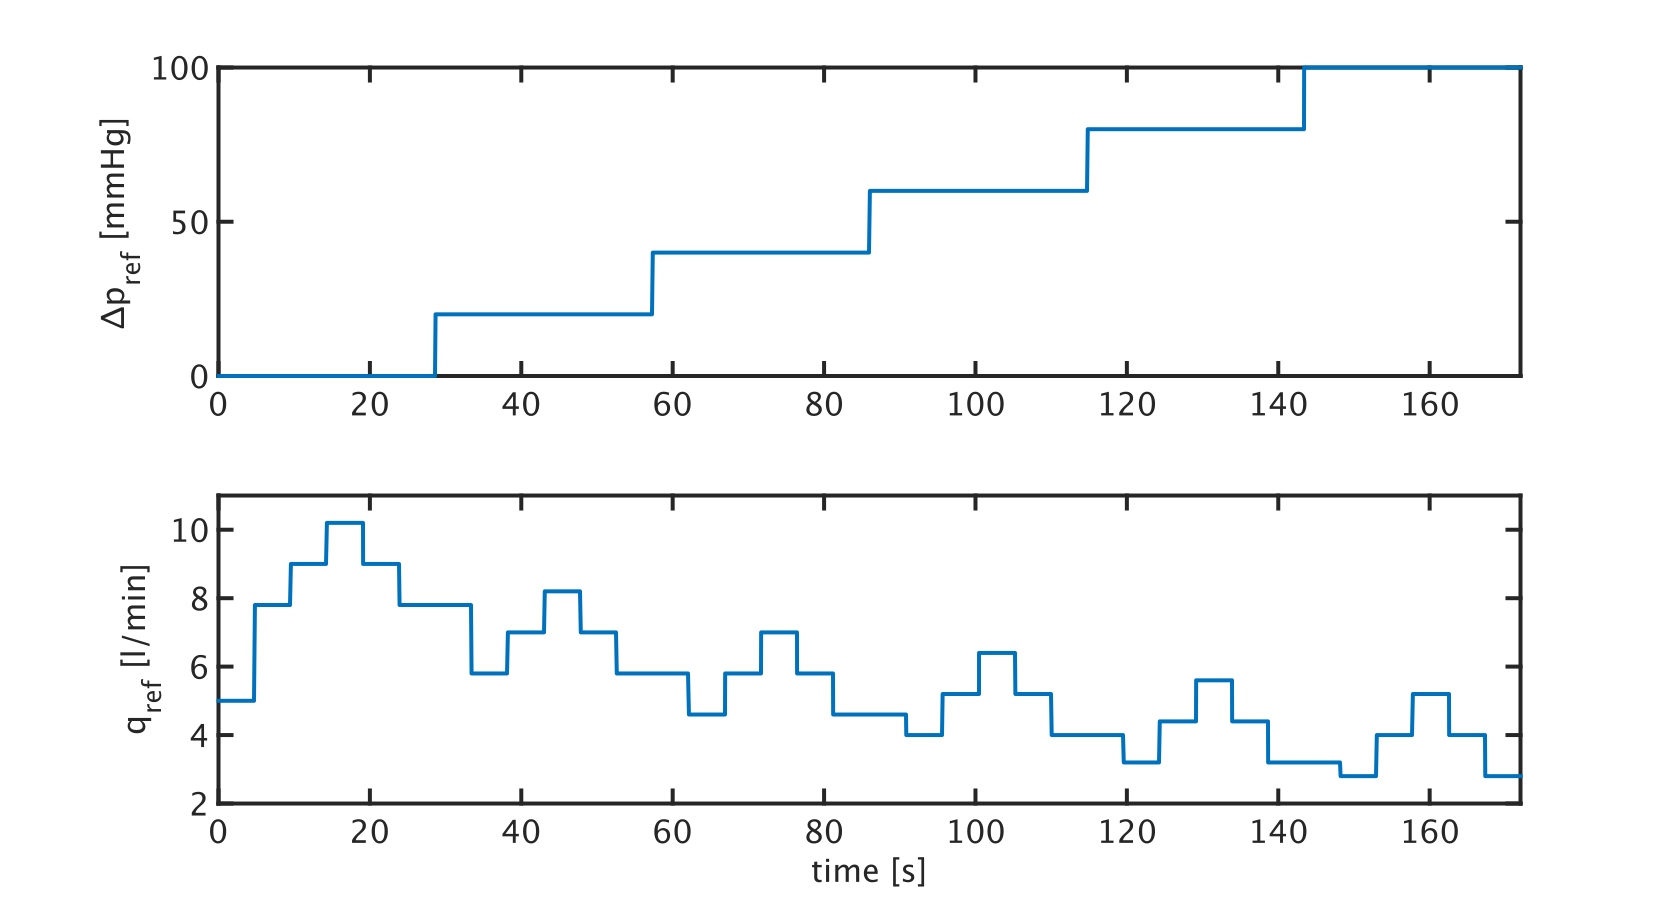
\includegraphics[width=\textwidth]{images/chapt_5/PI_control_ref_signals.pdf}
  \caption[Reference signals for PI controller performance evaluation]{Reference signals for PI controller performance evaluation. Top: differential pressure reference value. Bottom: targeted flow trajectory.}
  \label{fig:PI_control_ref_signals}
\end{figure}
\figurename~\ref{fig:pi_contr_chr_40} depicts the differential pressure and flow reference values, the measured pressure and flow value and the actuation variable in form of the reference rotational speed $v_{act}$ and rotational speed of the VAD $v_{vad}$ for the differential pressure level $\Delta{p}=40\,mmHg$ using the PI controller tuned according to Chien Hrones Reswick.
\begin{figure}[ht]
  \centering
  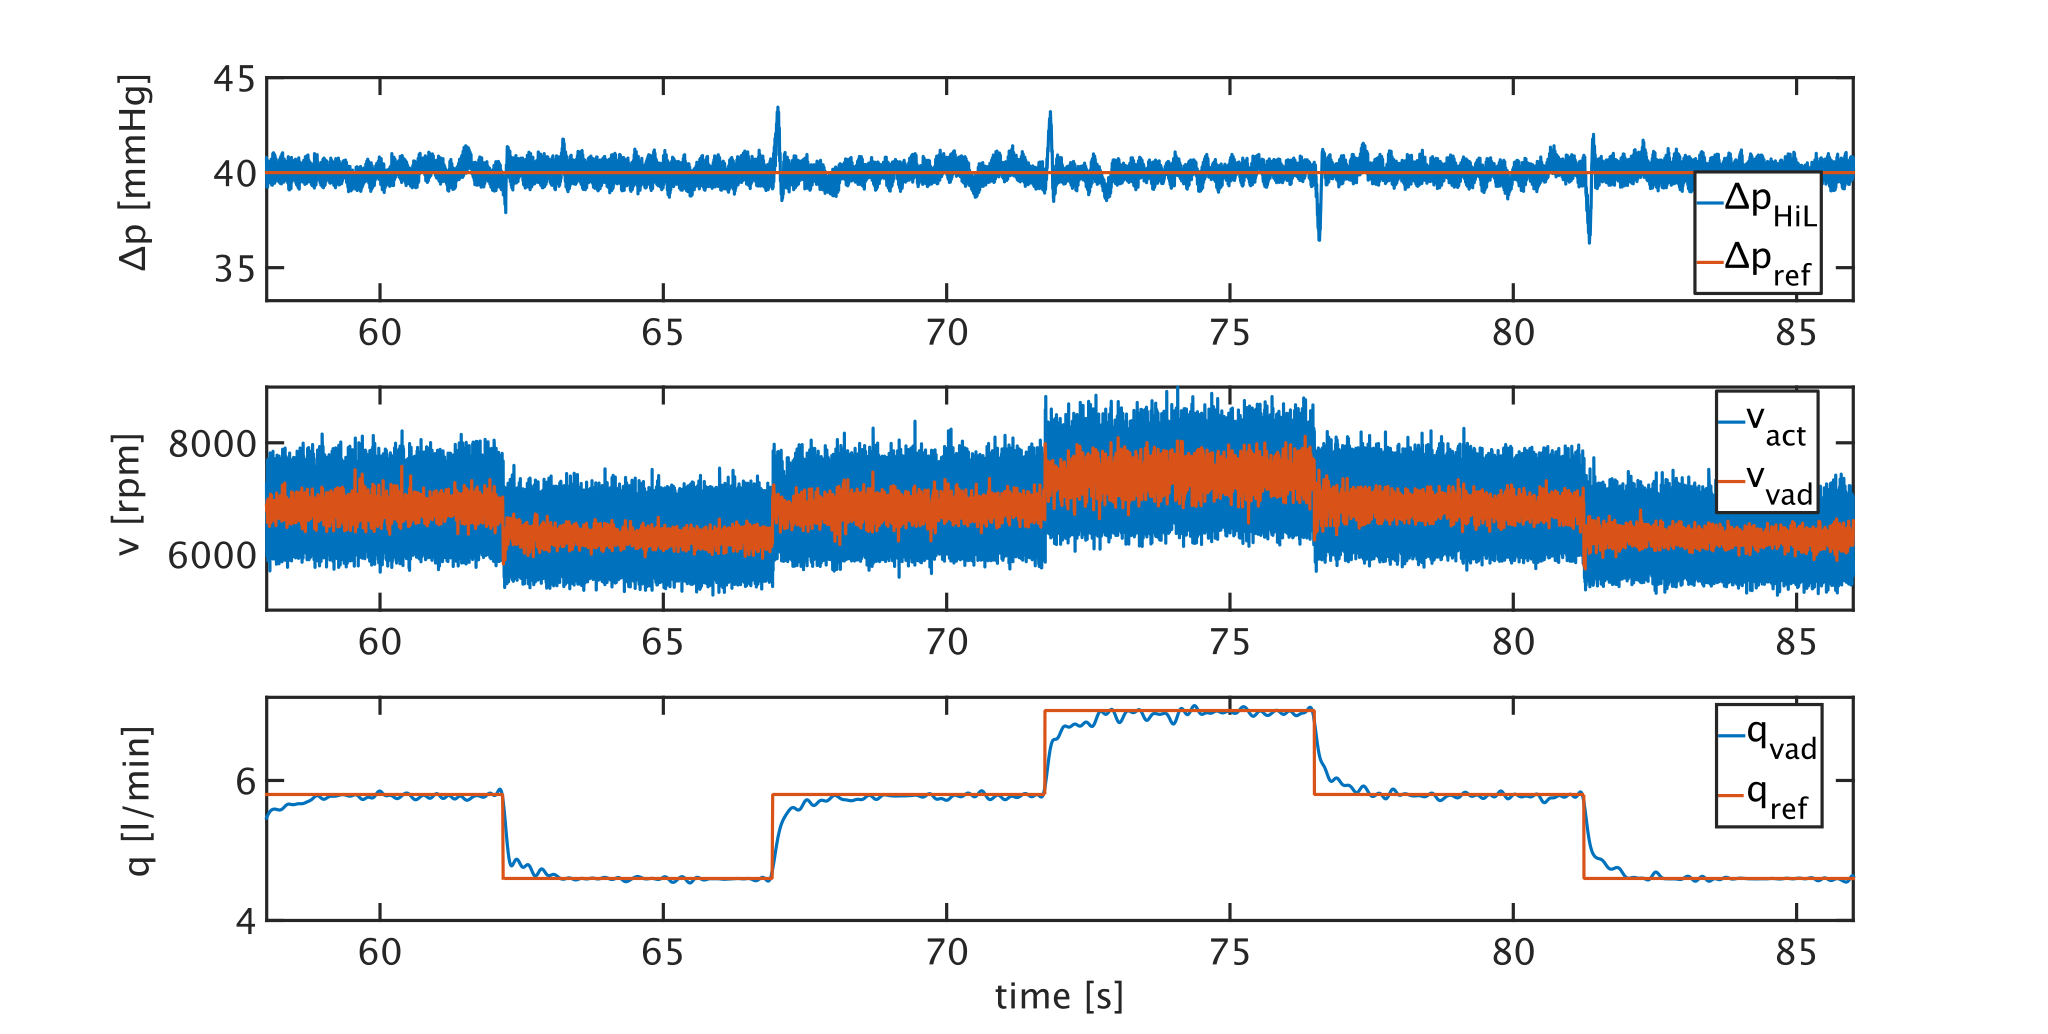
\includegraphics[width=0.9\textwidth]{images/chapt_5/pi_contr_chr_40.pdf}
  \caption[Test measurement for PI controller tuned according to Chien Hrones Reswick at $\Delta{p}=40\,mmHg$]{Test measurement for PI controller tuned according to Chien Hrones Reswick at $\Delta{p}=40\,mmHg$.}
  \label{fig:pi_contr_chr_40}
\end{figure}
\\The complete signal curves for the tests of the controllers are depicted in \figurename~\ref{fig:anh_6} and \figurename~\ref{fig:anh_7} in the appendix. Furthermore, the graphical representation of the test measurement at $\Delta{p}=40\,mmHg$ for the controller tuned according to Ziegler Nichols is depicted in \figurename~\ref{fig:anh_8} of the appendix.
\\The course of the control error throughout the test measurements of the controller tuned according to Ziegler Nichols and the controller tuned according to Chien Hrones Reswick are depicted in \figurename~\ref{fig:PI_error_a} and \figurename~\ref{fig:PI_error_b}, respectively.
\begin{figure}[ht]
  \centering
  \subfloat[]
  {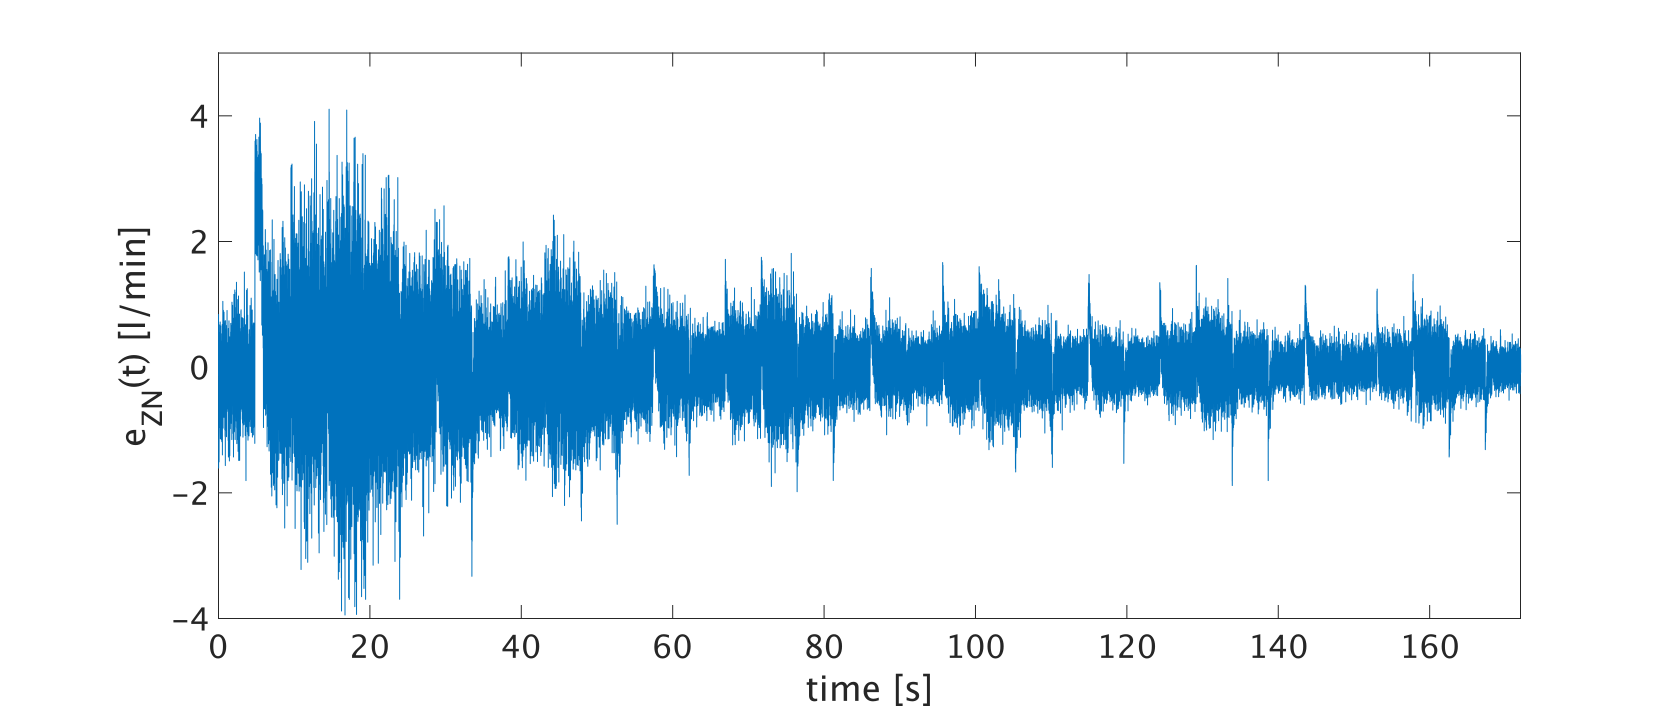
\includegraphics[width=0.5\textwidth]{images/chapt_5/error_PI_zn.pdf}\label{fig:PI_error_a}}
  \subfloat[]
  {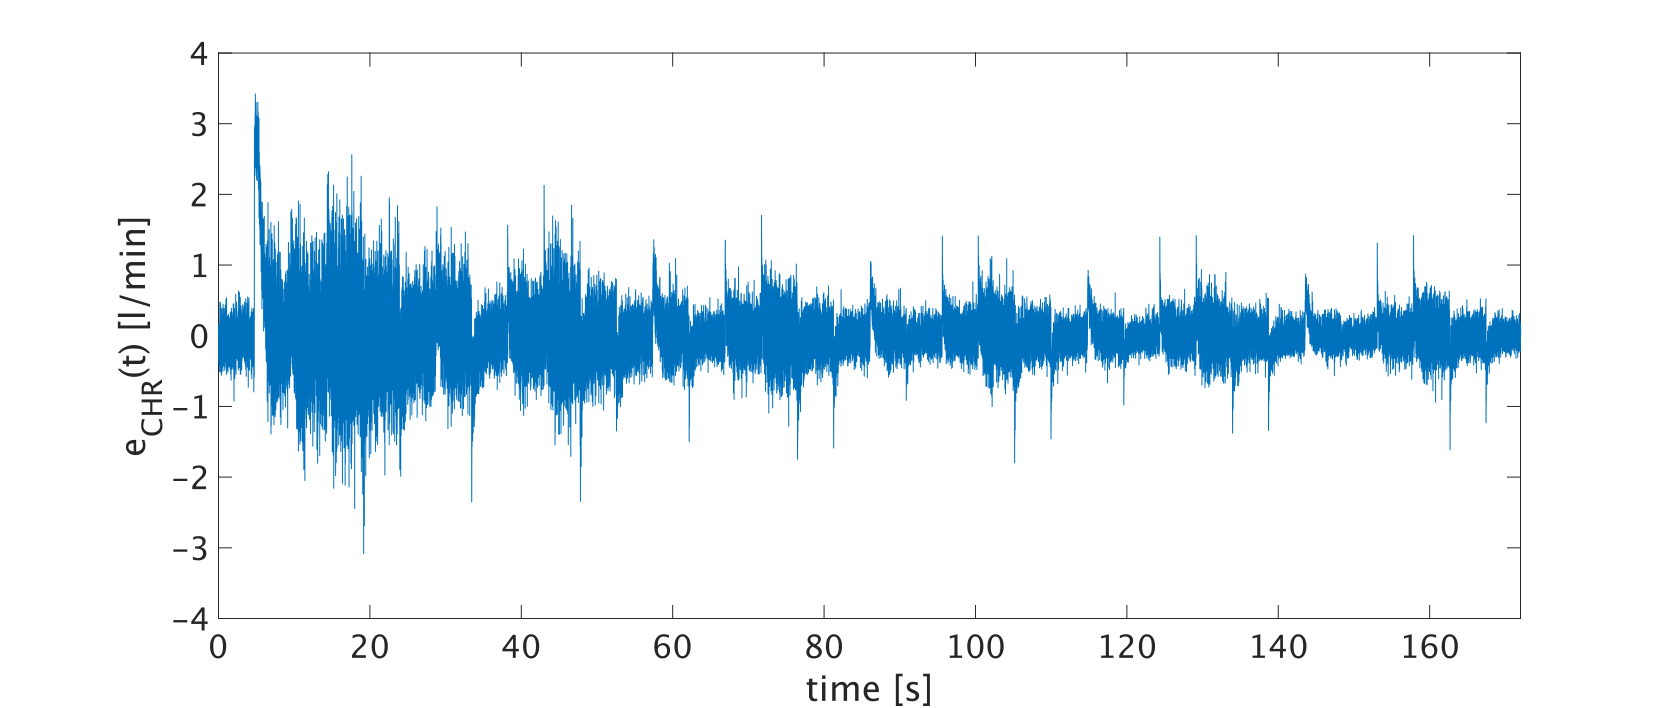
\includegraphics[width=0.5\textwidth]{images/chapt_5/error_PI_chr.pdf}\label{fig:PI_error_b}}
  \caption[Controll error for PI Controllers]{Controll error for PI controllers tuned according to (a) Ziegler Nichols, (b) Chien Hrones Reswick}
  \label{fig:PI_error}
\end{figure}
\\Throughout this work, for evaluation of controller performance the root mean square error (RMSE), according to \cite{RMSE}, defined as
\begin{equation}
  RMSE = \sqrt{\frac{1}{n}\sum_{i=0}^n e_i^2}
\end{equation}
is used. The RMSE for the differential pressure level of $\Delta{p}=40\,mmHg$ for Ziegler Nichols tuned controller amounts to
\begin{equation}
  RMSE_{ZN,40}=0.4013
\end{equation}
while RMSE of the second controller amounts to
\begin{equation}
  RMSE_{CHR,40}=0.2753.
\end{equation}
Taking into account the full differential pressure operating range for RMSE calculation these values amount to
\begin{equation}
  RMSE_{ZN}=0.5396
\end{equation}
and
\begin{equation}
  RMSE_{CHR}=0.3705.
\end{equation}
Comparing these results it is evident that both controllers perform more precise in the range of $\Delta{p}=40\,mmHg$, for which tuning has been performed.
Performance of the controller tuned according to Chien Hrones Reswick surpasses the Ziegler Nichols tuned one in both ranges. RMSE values for full range CHR control even indicate a higher performance in comparison to the Ziegler Nichols tuned controller in the range of $\Delta{p}=40\,mmHg$.
\\ Due to its higher performance, for all following measurements the PI controller tuned in reference to Chien Hrones Reswick is used.
\section{Iterative Learning Control}
As shown in \figurename~\ref{fig:pi_contr_chr_40}, the exclusive use of a PI controller for flow control leads to necessity of long measurement times to allow the flow to settle at a new reference value. However, one goal of this thesis is to enable flow control following different reference trajectories which may imply the need for faster reference tracking. By implementing an ILC approach, the necessary reduction of the settling time, by gaining information from error values of the preceding iteration, should be made possible.
\subsection{Design and Implementation}
During this work a P-type ILC is implemented and optimized.
\\The implementation is based on a parallel architecture as depicted in \figurename~\ref{fig:ILC_parallel}. This leads to the basic learning function for this ILC being represented by
\begin{equation}
  u_{j+1}(k) = u_{j}(k)+k_{p}e_{j}(k).
\end{equation}
The learning gain $k_p$ is experimentally chosen as
\begin{equation}
  k_p = 225
\end{equation}
to ensure quick error convergence.
\\As described in chapter \ref{ILC}, the basic ILC is extended to include a Q-Filter to enable more precise tuning of the ILC and increase its robustness.
This expansion results in the learning function being described by
\begin{equation}
  u_{j+1}(k) = Q(q)[u_{j}(k)+k_{p}e_{j}(k)].
\end{equation}
The Q-Filter is implemented as a $2^{nd}$-order butterworth filter, with sampling frequency $f_s=1000\,Hz$. The cut off frequency $f_c$ is set to several values in order to compare and thus optimize performance and robustness of the iterative learnig control system.
\\An additional part of the implementation is the generation of a repeating reference signal. 

\begin{figure}[ht]
  \centering
  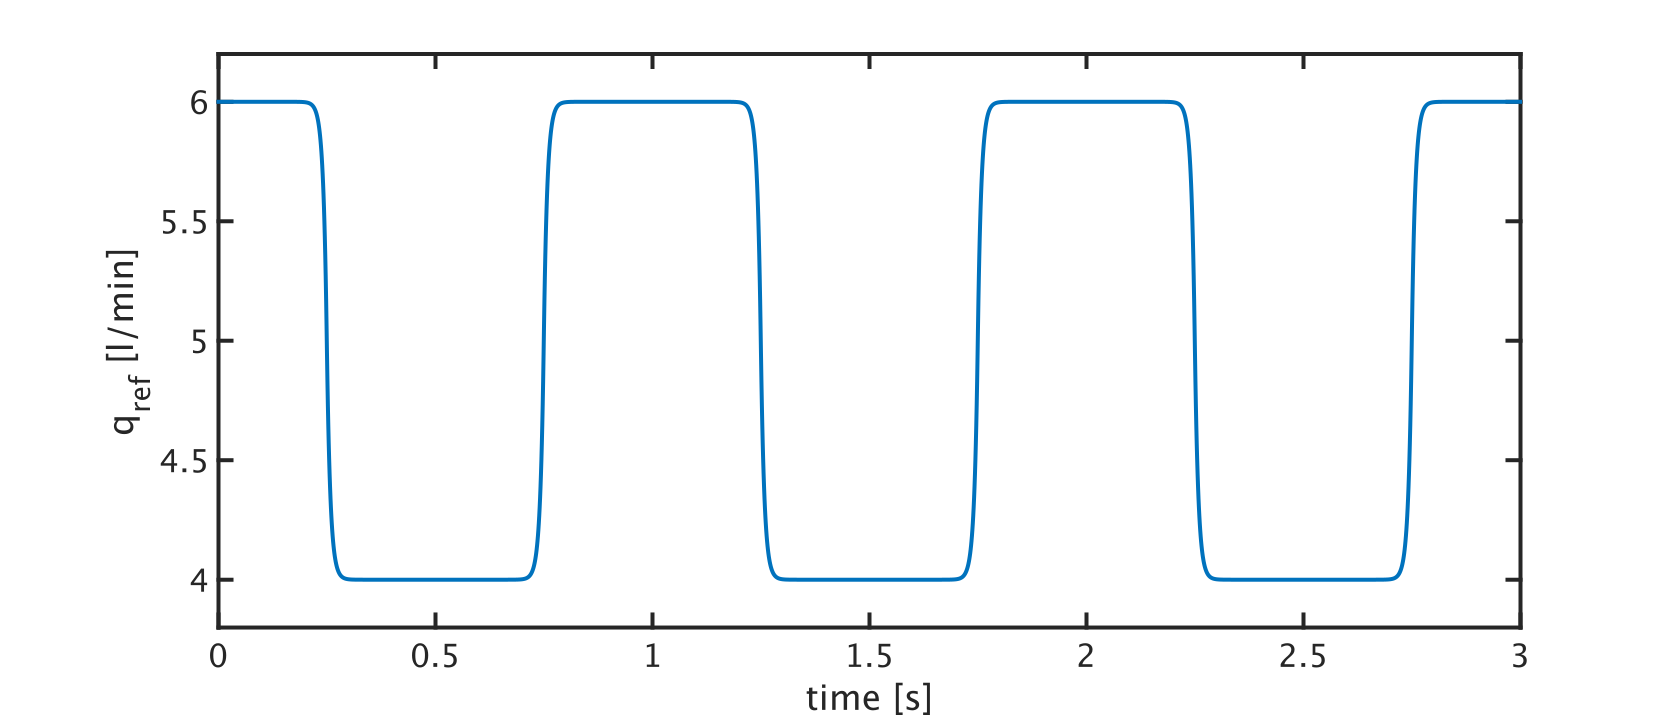
\includegraphics[width=\textwidth]{images/chapt_5/ILC/ref_signal_ILC3.pdf}
  \caption[Comparison of RMSE values for different cut off frequency of ILC Q-Filter]{Comparison of RMSE values for different cut off frequency of ILC Q-Filter.}
  \label{fig:ref_signal_ILC3}
\end{figure}
%Trigger signal aus simulink generiert
\subsection{Evaluation}


\begin{figure}[ht]
  \centering
  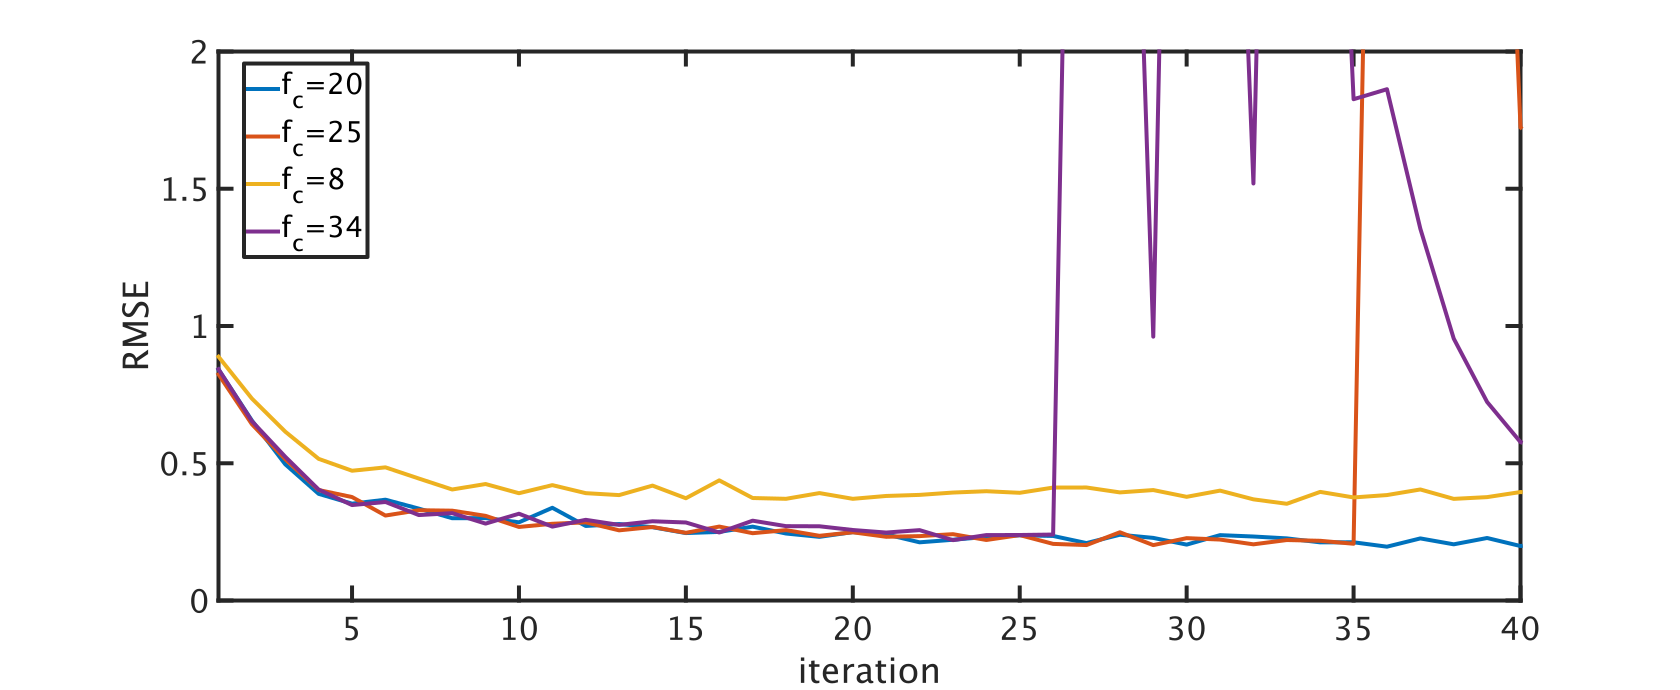
\includegraphics[width=\textwidth]{images/chapt_5/ILC/RMSE_compare_ILC3_fc.pdf}
  \caption[Comparison of RMSE values for different cut off frequency of ILC Q-Filter]{Comparison of RMSE values for different cut off frequency of ILC Q-Filter.}
  \label{fig:RMSE_compare_ILC3_fc}
\end{figure}
\section{Iterative Learning Control with repeating disturbance}
%trigger von Stoerung
\subsection{Design and Implementation}

\subsection{Evaluation}
%Q Filter optimierung f c vergleich
%Test auf verschiedenen Arbeitsbereichen
\section{Iterative Learning Control with varying disturbance length}
%trigger von Stoerung
\subsection{Design and Implementation}
\subsection{Evaluation}
% \section{Evaluation}
% \subsection{PI Controller}
% % gesamt:
% % rms pi total chr = 0.3705
% % rms pi total zn = 0.5396
% % \begin{figure}[ht]
% %   \centering
% %   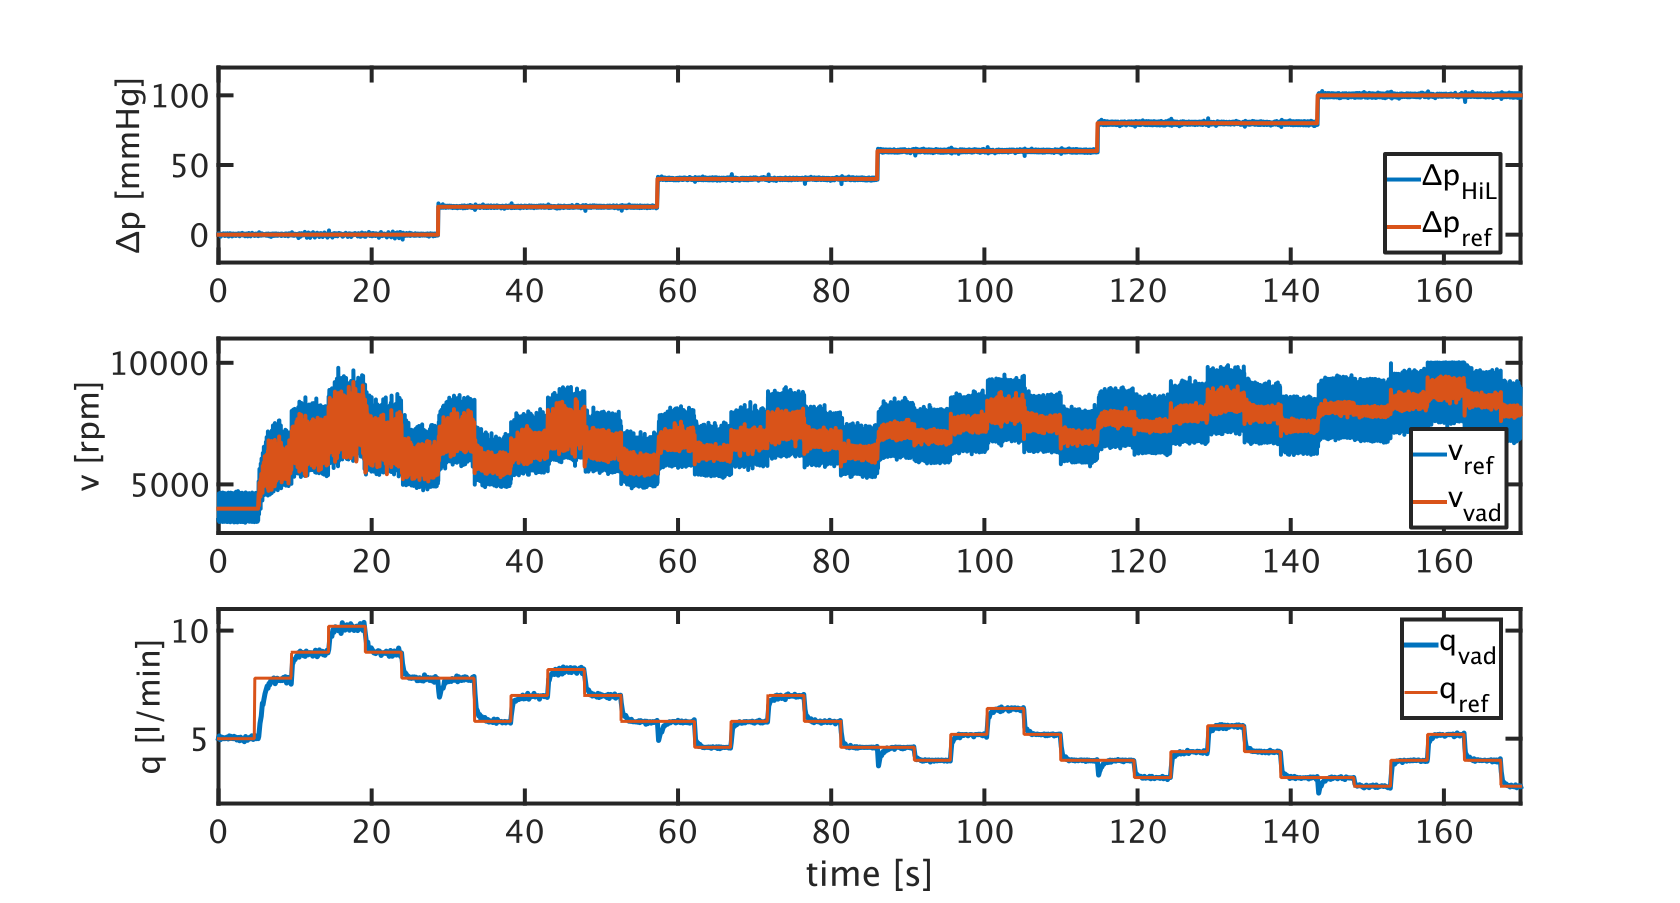
\includegraphics[width=\textwidth]{images/chapt_5/pi_contr_chr.pdf}
% %   \caption[Step response for determination of PI controller tuning parameters]{Step response for a step in rotational speed of $400\,rpm$ for determination of PI controller tuning parameters.}
% %   \label{fig:pi_contr_chr}
% % \end{figure}
%
% % \begin{figure}[ht]
% %   \centering
% %   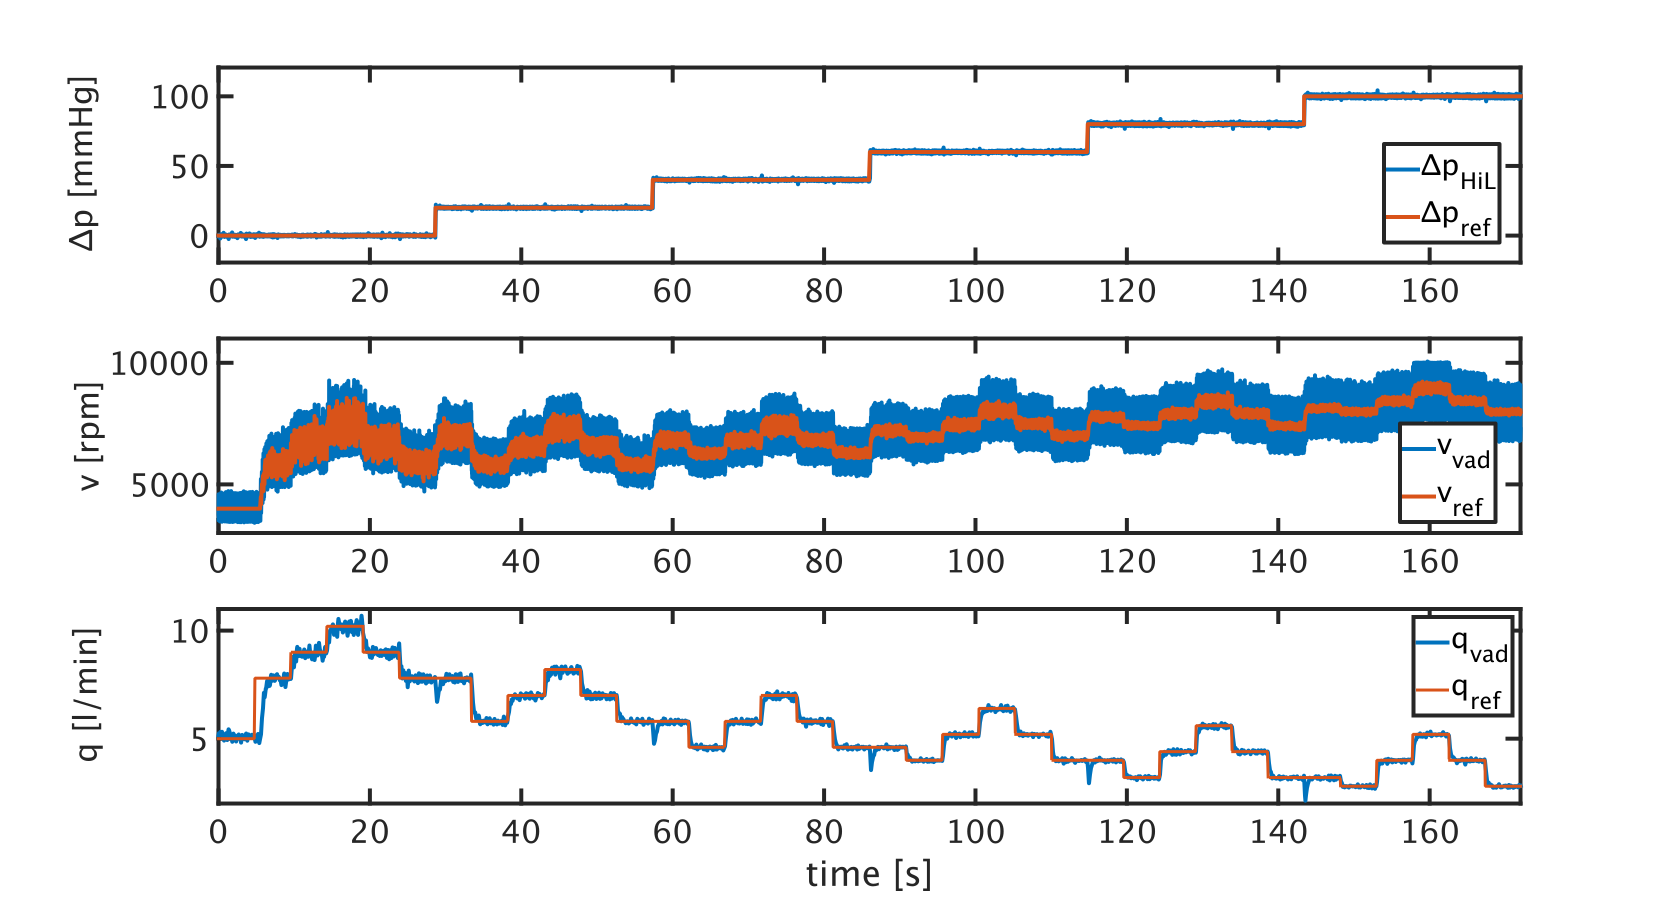
\includegraphics[width=\textwidth]{images/chapt_5/pi_contr_zn.pdf}
% %   \caption[Step response for determination of PI controller tuning parameters]{Step response for a step in rotational speed of $400\,rpm$ for determination of PI controller tuning parameters.}
% %   \label{fig:pi_contr_zn}
% % \end{figure}
%
% % Bereich der Auslegung: 40mmHg
% % RMS PI CHR = 0.2753
% % RMS PI ZN = 0.4013
%
% % \begin{figure}[ht]
% %   \centering
% %   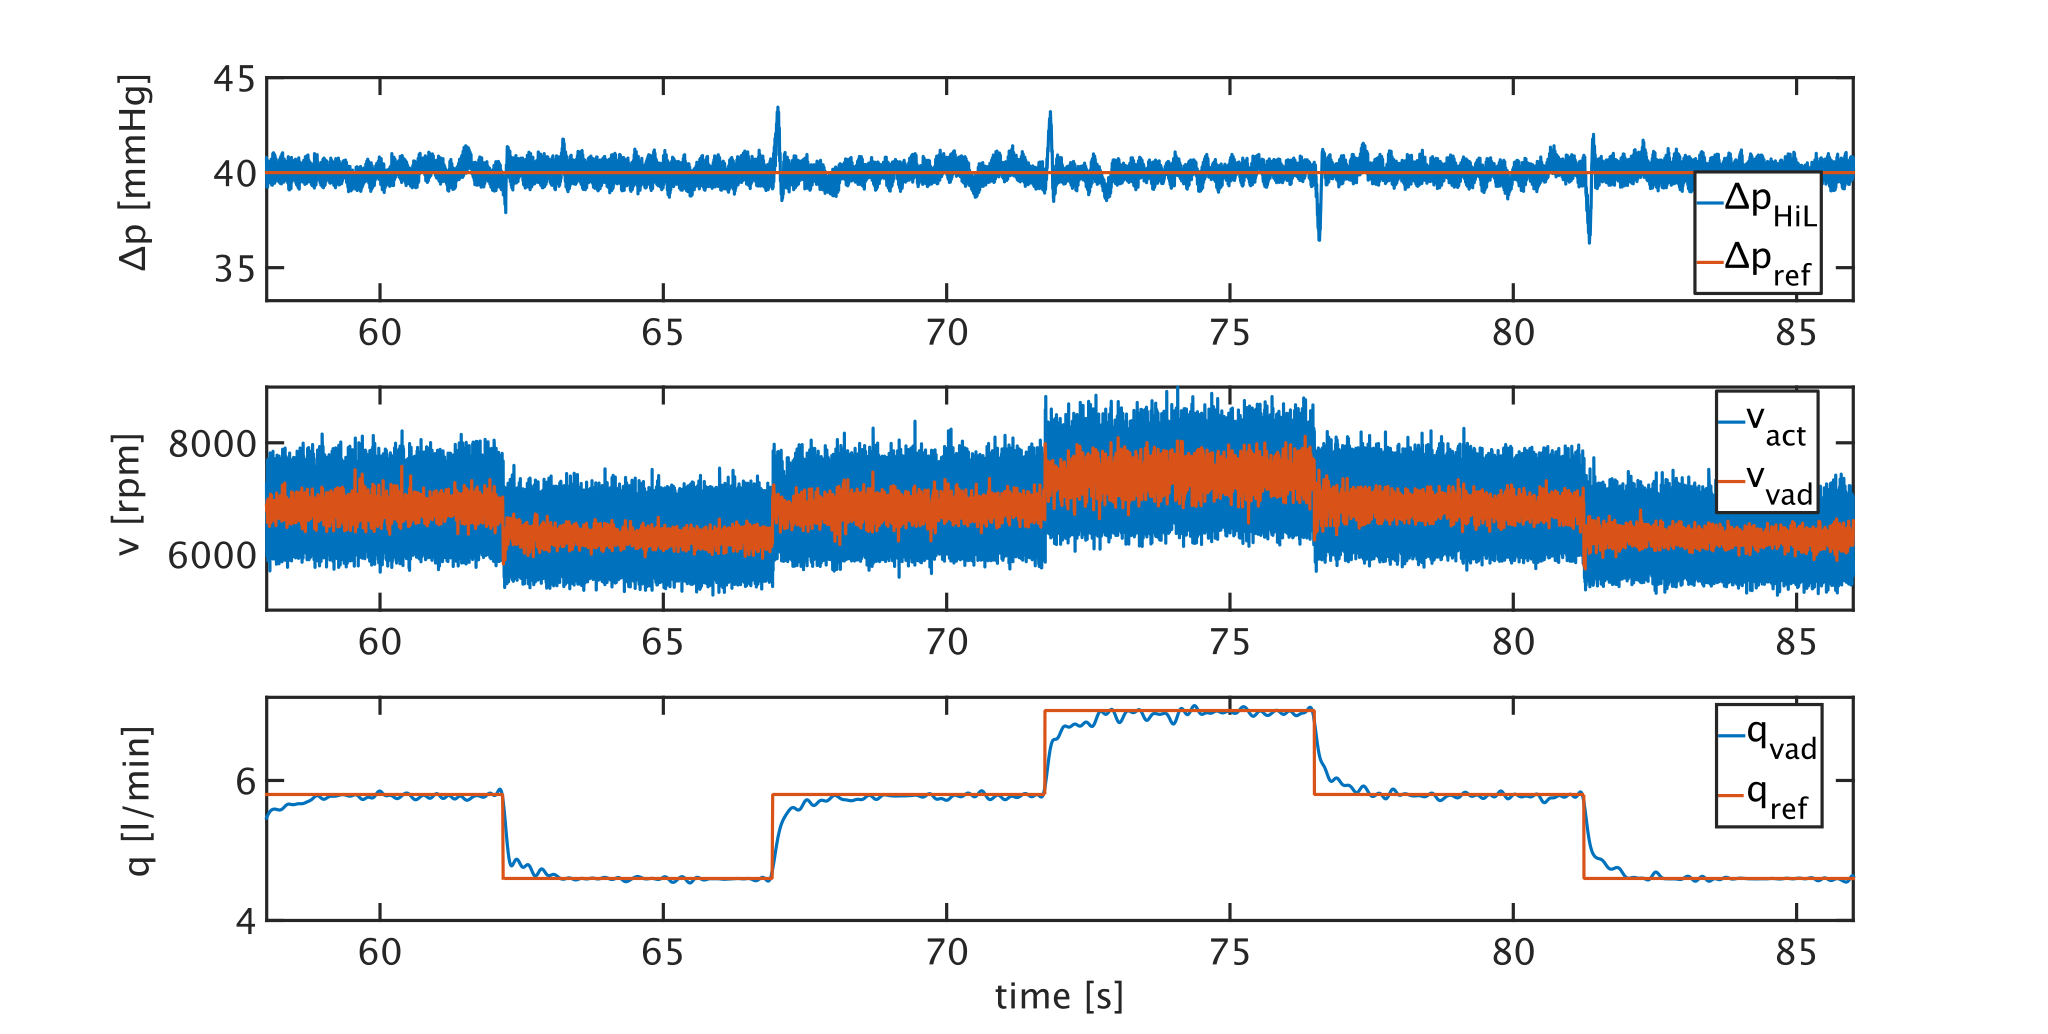
\includegraphics[width=\textwidth]{images/chapt_5/pi_contr_chr_40.pdf}
% %   \caption[Step response for determination of PI controller tuning parameters]{Step response for a step in rotational speed of $400\,rpm$ for determination of PI controller tuning parameters.}
% %   \label{fig:pi_contr_chr_40}
% % \end{figure}
%
% % \begin{figure}[ht]
% %   \centering
% %   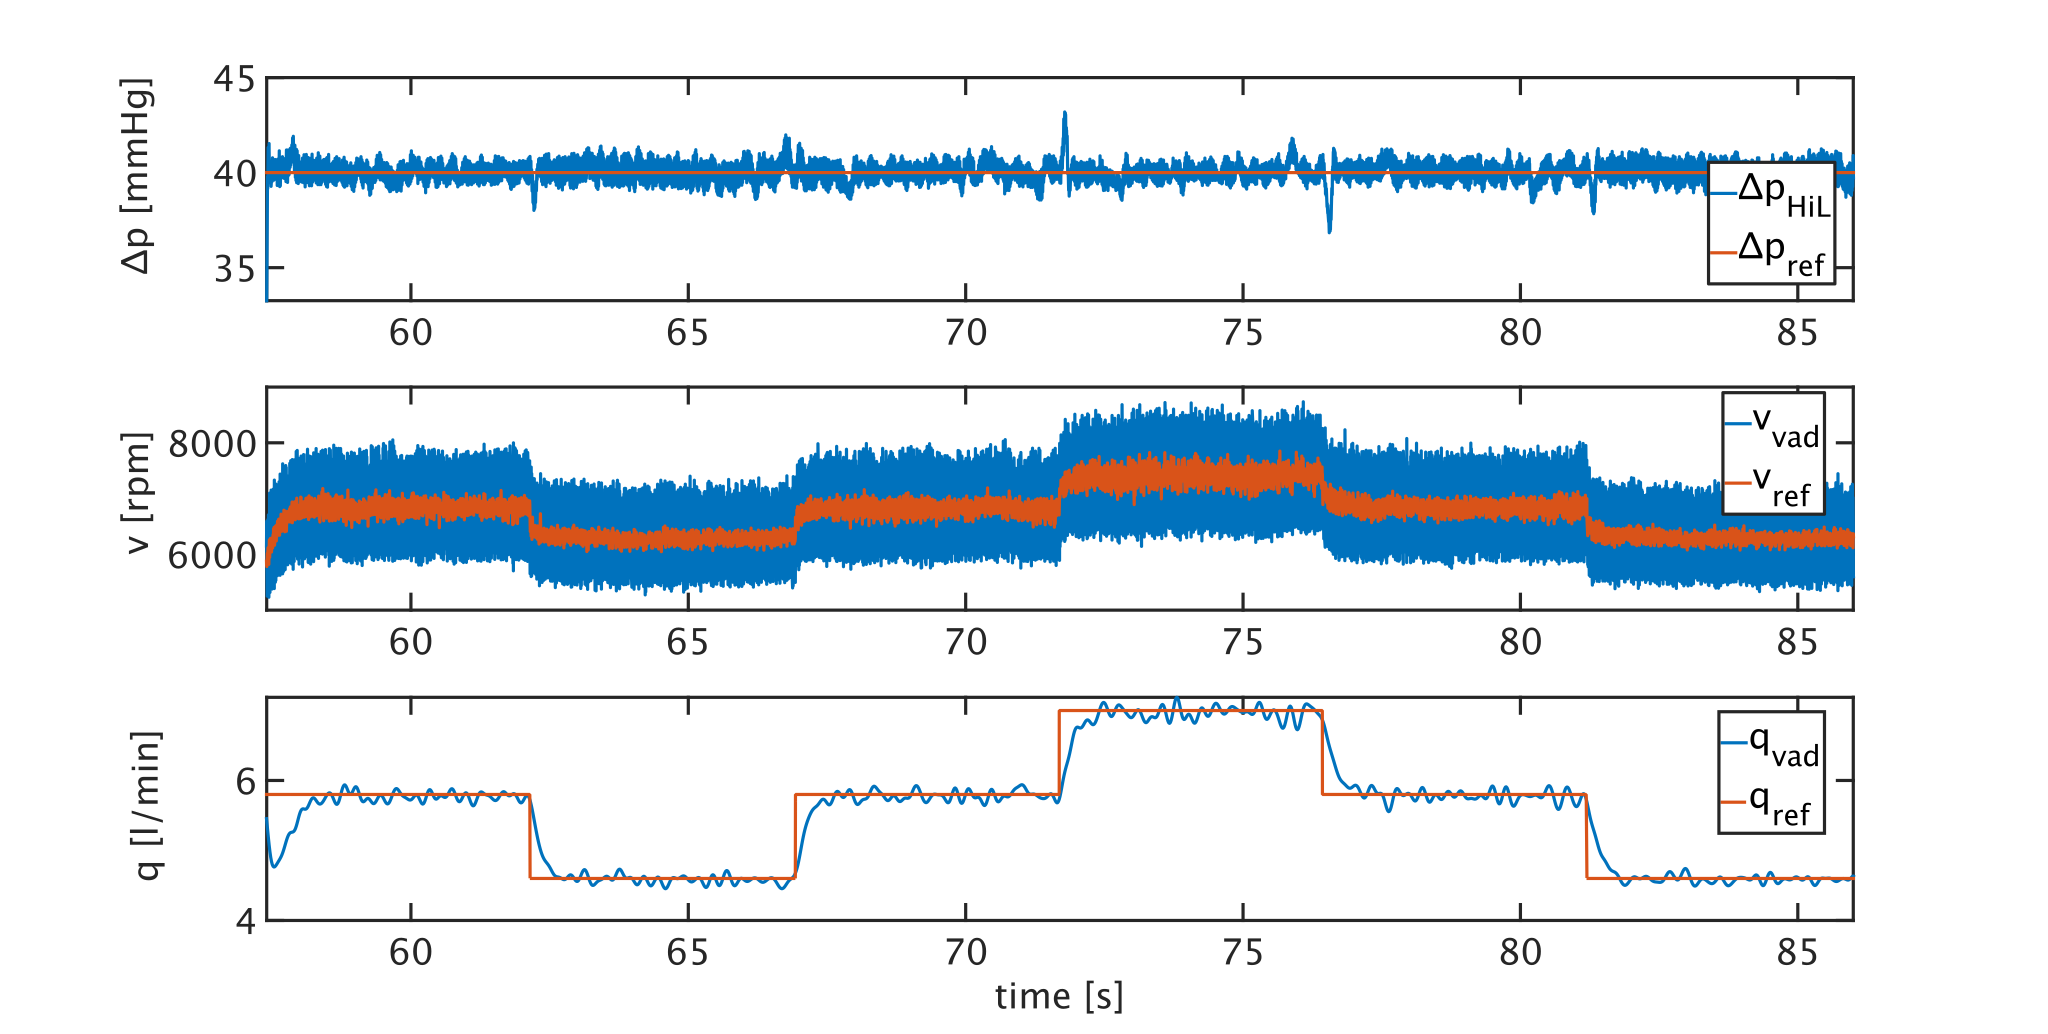
\includegraphics[width=\textwidth]{images/chapt_5/pi_contr_zn_40.pdf}
% %   \caption[Step response for determination of PI controller tuning parameters]{Step response for a step in rotational speed of $400\,rpm$ for determination of PI controller tuning parameters.}
% %   \label{fig:pi_contr_zn_40}
% % \end{figure}
%
% % Dynamische Messung nutzen
% % Werte an Sprungstellen
% % Nach Wendetangenten verfahren -> GRAFIK
% %Berechnung erklären
% \subsection{Iterative Learning Control}
% \subsection{Iterative Learning Control with varying iteration length}
% % Kontanten Fluss über verschiedene Druckbereiche?
% %
% % %Druckverlauf ohne Störung
% %
% % Herzschlag dazu - Druckverlauf
